\subsubsection{\textit{Lưu đồ thuật toán (Flowchart)}}

\vspace{0.5cm}
\noindent\textbf{\Large Flowchart của thuật toán:} Hình~\ref{fig:flowchart-group}

\vspace{0.3cm}
\begin{figure}[H]
    \centering
    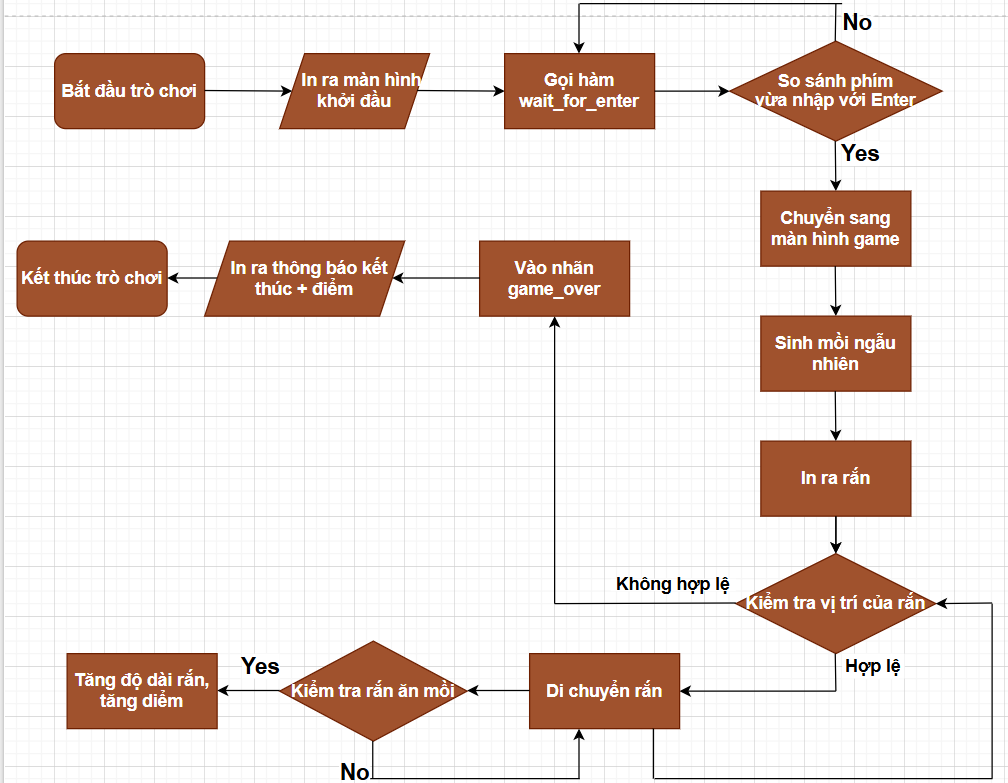
\includegraphics[width=0.9\textwidth]{Images/Flowchart/Flowchart-group.png}
    \caption{Flowchart Snake Game}
    \label{fig:flowchart-group}
\end{figure}

\vspace{0.4cm}
\noindent \textbf{Trong đó:}
\begin{itemize}
    \itemsep0.2cm
    \item \textbf{Dữ liệu đầu vào:} Người dùng nhập phím \texttt{\textbf{Enter}} để bắt đầu trò chơi, sử dụng các phím mũi tên \texttt{\textbf{↑ ↓ ← →}} để điều khiển rắn di chuyển.
    \item \textbf{Dữ liệu đầu ra:} Khi bắt đầu, in ra tên trò chơi và thông báo yêu cầu người dùng nhập \texttt{\textbf{Enter}} để chơi. Khi kết thúc, in ra thông báo \texttt{\textbf{"Game Over"}} và điểm của người chơi.
\end{itemize}

\subsubsection{\textit{Phân tích chi tiết}}
\vspace{0.5cm}

\noindent \textbf{Mã nguồn chi tiết của thuật toán tại:} \href{http://bit.ly/3GG2OQN}{\texttt{\large http://bit.ly/3GG2OQN}}

\vspace{0.5cm}
\noindent\textbf{\Large Phân tích chương trình:}
\vspace{0.3cm}

\begin{lstlisting}[style=asm]
    .model small
    .stack 100h
    .data
        snake dw 10Dh, 10Ch, 10Bh, 10Ah, 150 dup(?) 
        s_size db 4,0     
        tail dw ?         
        
        left  equ 4Bh  
        right equ 4Dh   
        up    equ 48h
        down  equ 50h
    
        cur_dir db right  
        old_dir db right    
        
        mealX db ?
        mealY db ?
    
        score db '0','0','0','0','$' 
        
        ;2 bien msgstart va msgover nhu hinh duoi
    .code
\end{lstlisting}

\vspace{0.4cm}
\begin{figure}[H]
    \centering
    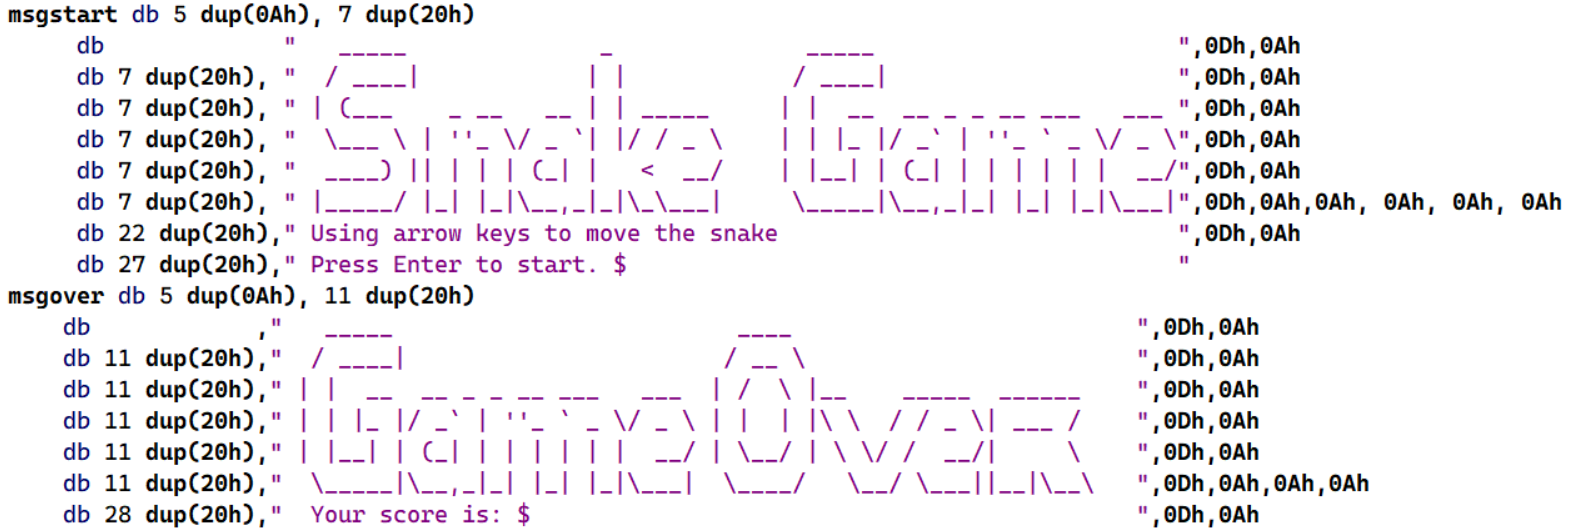
\includegraphics[width=0.9\textwidth]{Images/CodeSample/Code-1.png}
    \caption{Biến \texttt{msgstart} và \texttt{msgover}}
    \label{fig:codesample-1}
\end{figure}

\vspace{0.4cm}
\noindent \textbf{Trong đoạn code trên:}
\begin{itemize}
    \itemsep0.2cm
    \item \textbf{\texttt{.model small}}: chọn mô hình bộ nhớ "small", nghĩa là segment code và data riêng biệt, mỗi segment tối đa 64KB.
    \item \textbf{\texttt{.stack 100h}}: đặt vùng stack có kích thước 256 bytes (100h = 256).
    \item \textbf{\texttt{.data}}: bắt đầu khai báo biến.
    \item \textbf{\texttt{snake}}: khai báo con rắn ban đầu có 4 ô từ (10,1) đến (13,1), có 150 ô trống để thêm khi rắn ăn được mồi.
    \item \textbf{\texttt{s\_size}}: lưu độ dài rắn, ban đầu là 4.
    \item \textbf{\texttt{tail}}: lưu vị trí đuôi rắn.
    \item \textbf{\texttt{left, right, up, down}}: định nghĩa các biến ứng với phím mũi tên trên bàn phím.
    \item \textbf{\texttt{cur\_dir}}, \textbf{\texttt{old\_dir}}: lưu hướng hiện tại và hướng cũ của rắn, mặc định ban đầu là \texttt{right}.
    \item \textbf{\texttt{mealX}}, \textbf{\texttt{mealY}}: lưu tọa độ X, Y của mồi.
    \item \textbf{\texttt{score}}: lưu điểm của người chơi, tối đa 4 chữ số.
    \item \textbf{\texttt{msgstart}}: lưu nội dung màn hình bắt đầu.
    \item \textbf{\texttt{msgover}}: lưu nội dung khi trò chơi kết thúc.
\end{itemize}

\vspace{0.5cm}

\begin{lstlisting}[style=asm]
    main proc
    mov ax, @data
    mov ds, ax
                                     
    mov ah, 9   
    lea dx, msgstart                             
    int 21h  
                                    
    mov ax, 40h   
    mov es, ax    

    call wait_for_enter     

    mov al, 1     
    mov ah, 5      
    int 10h            
    
    call randomizeMeal
\end{lstlisting}

\vspace{0.4cm}
\noindent \textbf{Trong đoạn code trên:}
\begin{itemize}
    \itemsep0.2cm
    \item \textbf{\texttt{main proc}}: bắt đầu hàm main.
    \item \textbf{\texttt{mov ax, @data} | \texttt{mov ds, ax}}: dùng thanh ghi \texttt{ax} làm trung gian để gán các giá trị trong \texttt{.data} vào thanh ghi \texttt{ds}.
    \item \textbf{\texttt{mov ah, 9} | \texttt{lea dx, msgstart} | \texttt{int 21h}}: sử dụng ngắt 9 để in ra màn hình biến msgstart.
    \item \textbf{\texttt{mov ax, 40h} | \texttt{mov es, ax}}: dùng thanh ghi \texttt{ax} làm trung gian để gán \texttt{40h} cho \texttt{es}, nhằm lưu các thông số dòng, cột của màn hình trò chơi.
    \item \textbf{\texttt{call} \texttt{wait\_for\_enter}}: gọi hàm \texttt{wait\_for\_enter}, hàm này có nội dung như sau:
    
    \vspace{0.3cm}
    \begin{lstlisting}[style=asm]
        wait_for_enter proc
            push ax 
            wait_loop:
                mov ah, 0      
                int 16h        
                cmp al, 13      
                jne wait_loop  
            pop ax
            ret
        wait_for_enter endp  
    \end{lstlisting}
    \vspace{0.3cm}

    \begin{itemize}
        \item \textbf{\texttt{push ax}}: đẩy thanh ghi \texttt{ax} vào \texttt{stack} để bảo toàn dữ liệu.
        \item \textbf{\texttt{wait\_loop}}: vào nhãn \texttt{wait\_loop}
        \item \textbf{\texttt{mov ah, 0} | \texttt{int 16h}}: dùng ngắt 0 nhập kí tự, không in lên màn hình.
        \item \textbf{\texttt{cmp al, 13}}: so sánh kí tự vửa nhập với kí tự \texttt{Enter}.
        \item \textbf{\texttt{jne} \texttt{wait\_loop}}: nếu không phải là kí tự \texttt{Enter} thì tiếp tục lặp.
        \item \textbf{\texttt{pop ax} | \texttt{ret}}: trả lại giá trị cho thanh ghi \texttt{ax} và kết thúc hàm.
    \end{itemize}
    
    \item \textbf{\texttt{mov al, 1} | \texttt{mov ah, 5} | \texttt{int 10h}}: chuyển sang trang màn hình mới.
    \item \textbf{\texttt{call randomizeMeal}}: gọi hàm \texttt{randomizeMeal}, hàm này có nội dung như sau:
    
    \vspace{0.3cm}
    \begin{lstlisting}[style=asm]
        randomizeMeal proc
            mov ah, 00h  
            int 1ah      
                
            mov ax, dx     
            xor dx, dx     
            mov cx, 25      
            div cx         
            mov mealY, dl   
                
            mov ah, 00h    
            int 1ah 
                
            mov ax, dx      
            xor dx, dx
            mov cx, 80       
            div cx
            mov mealX, dl    
                
            mov dh, mealY      
            mov cx, w.s_size    
            xor bx, bx          
            
            check_snake:
                cmp dx, snake[bx]     
                je randomizeMeal      
                    
                add bx, 2             
                loop check_snake      
                
            mov ah, 02h         
            mov bh, 01h         
            int 10h
                
            mov al, 04h        
            mov bl, 0eh        
            mov cx, 1         
            mov ah, 09h        
            int 10h 
                
            ret
        randomizeMeal endp                              
    \end{lstlisting}
    \vspace{0.3cm}

    \begin{itemize}
        \item \textbf{\texttt{mov ah, 00h} | \texttt{int 1ah} | \texttt{mov ax, dx} | \texttt{xor dx, dx}}: lấy 1 giá trị ngẫu nhiên, dùng \texttt{dx} làm trung gian để lưu giá trị đó vào \texttt{ax}, sau đó gán lại \texttt{dx} = 0.
        \item \textbf{\texttt{mov cx, 25} | \texttt{div cx} | \texttt{mov mealY, dl}}: lấy giá trị ngẫu nhiên vừa có chia cho 25 (số dòng) rồi gán cho \texttt{mealY}.
        \item 7 dòng code tiếp theo: tương tự như \texttt{mealY}, tính và gán giá trị cho \texttt{mealX}.
        \item \textbf{\texttt{mov dh, mealY} | \texttt{mov cx, w.}\texttt{s\_size} | \texttt{xor bx, bx}}: gán tọa độ của mồi vào \texttt{dx}, chiều dài rắn vào \texttt{cx}, đưa \texttt{bx} về 0 để trỏ vào đoạn đầu của rắn.
        \item \textbf{\texttt{check\_snake}}: vào nhãn \texttt{check\_snake}.
        \item \textbf{\texttt{cmp dx, snake[bx]} | \texttt{je randomizeMeal}}: so sánh vị trí mồi với từng đoạn của rắn, nếu trùng nhau thì tạo lại mồi.
        \item \textbf{\texttt{add bx, 2} | \texttt{loop} \texttt{check\_snake}}: nếu không trùng nhau thì kiểm tra đến đoạn tiếp theo của con rắn.
        \item Các dòng code còn lại: in ra mồi trên màn hình.
    \end{itemize}

\begin{lstlisting}[style=asm]
    game_loop:
        call shownewhead
    
        mov dx, snake[0]     
        mov si, w.s_size    
        add si, w.s_size    
        sub si, 2            
        mov cx, w.s_size    
        sub cx, 4
        jz no_death          
    deathloop:              
        cmp dx, snake[si]    
        je game_over
        sub si, 2           
        dec cx               
        jnz deathloop        
    no_death:
        mov si, w.s_size     
        add si, w.s_size
        sub si, 2
        mov ax, snake[si]    
        mov tail, ax
    
        call move_snake             
    
        mov dx, snake[0]          
        mov al, mealX             
        mov ah, mealY
        cmp ax, dx                
        jne hide_old_tail         
        mov al, s_size            
        inc al
        mov s_size, al            
        mov ax, tail             
        mov bh, 0
        mov bl, s_size           
        add bl, s_size            
        sub bl, 2
        mov snake[bx], ax           
        call scoreplus              
        call randomizeMeal          
        jmp no_hide_old_tail       
    
    hide_old_tail:
        mov dx, tail            
        
        mov ah, 02h              
        int 10h
    
        mov al, ' '              
        mov ah, 09h              
        mov bl, 0Fh
        mov cx, 1     
        int 10h  
        
    no_hide_old_tail:
        mov ah, 01h             
        int 16h
        jz no_key
    
        mov ah, 00h           
        int 16h                 
        cur_dir
        mov cur_dir, ah
    
    no_key:
        jmp game_loop           
\end{lstlisting}

\vspace{0.5cm}
\noindent \textbf{Trong đoạn code trên:}
\begin{itemize}
    \itemsep0.3cm
    \item \textbf{\texttt{call shownewhead}: gọi đến hàm \texttt{shownewhead} có nội dung như sau}:
    
    \vspace{0.3cm}
    \begin{lstlisting}[style=asm]
        shownewhead proc
            mov dx, snake[0]      
            
            mov ah, 02h        
            int 10h            
            
            mov al, 002        
            mov ah, 09h       
            mov bl, 0Ah
            mov bh, 01h
            mov cx, 1
            int 10h 
            
            ret
        shownewhead endp                          
    \end{lstlisting}
    \vspace{0.3cm}
    
    \begin{itemize}
        \itemsep0.2cm
        \item \textbf{\texttt{mov dx, snake[0]} | \texttt{mov ah, 02h} | \texttt{int 10h}}: lưu vị trí đoạn đầu của rắn vào \texttt{dx}, đồng thời di chuyển con trỏ đến vị trí đó.
        \item Các dòng code còn lại: hiển thị rắn lên màn hình (chiều dài mặc định là 4).
    \end{itemize}

    \item 5 dòng code tiếp theo: lưu độ dài của rắn và trỏ tới đuôi rắn.
    \item \textbf{\texttt{sub cx, 4} | \texttt{jz} \texttt{no\_death}}: Kiểm tra nếu độ dài rắn bằng 4 (độ dài mặc định) => rắn không thế chết, nhảy vào nhãn \texttt{no\_death}.
    \item \textbf{\texttt{deathloop}}: vào nhãn \texttt{deathloop}.
    \item \textbf{\texttt{cmp dx, snake[si]} | \texttt{je} \texttt{game\_over}}: Kiểm tra nếu đầu rắn và thân rắn trùng nhau => rắn chết, nhảy vào nhãn \texttt{game\_over}. Nhãn này có nội dung như sau:
    
    \vspace{0.3cm}
    \begin{lstlisting}[style=asm]
        game_over:
            xor dx, dx                      
            
            mov ah, 02h                   
            int 10h                  
            
            mov ah, 9                     
            lea dx, msgover  
            int 21h   
            
            mov ah, 9
            lea dx, score                   
            int 21h                   
    \end{lstlisting}
    \vspace{0.3cm}
    
    \begin{itemize}
        \itemsep0.2cm
        \item \textbf{\texttt{xor dx, dx}}: đặt lại \texttt{dx} = 0.
        \item \textbf{\texttt{mov ah, 02h} | \texttt{int 10h}}: đưa con trỏ về lại vị trí \texttt{dx}.
        \item Các dòng còn lại: in ra màn hình thông báo \texttt{Game Over} và điểm của người chơi.
    \end{itemize}

    \item 3 dòng tiếp theo: nếu không trùng nhau, nhảy đến các đoạn còn lại của rắn và tiếp tục kiểm tra.
    \item \textbf{\texttt{no\_death:}} vào nhãn \texttt{no\_death}.
    \item 5 dòng tiếp theo: xác định lại vị trí đuôi rắn (có thể bị thay đổi nếu nhảy vào \texttt{deathloop}), sau đó lưu vào \texttt{tail} qua thanh ghi \texttt{ax}.
    \item \textbf{\texttt{call} \texttt{move\_snake}}: vào hàm \texttt{move\_snake}. Hàm này có nội dung như sau:
    
    \vspace{0.3cm}
    \begin{lstlisting}[style=asm]
        move_snake proc
            mov di, w.s_size         
            add di, w.s_size
            sub di, 2
        
            mov cx, w.s_size         
            dec cx                   
        
            move_array:
                mov ax, snake[di-2]   
                mov snake[di], ax     
                sub di, 2            
                loop move_array       
            
            getdir:                     
                cmp cur_dir, left
                je move_left
                cmp cur_dir, right
                je move_right
                cmp cur_dir, up
                je move_up
                cmp cur_dir, down
                je move_down
            
            get_old_dir:               
                mov al, old_dir
                mov cur_dir, al
                jmp getdir 
                
            move_left:                   
                cmp old_dir, right      
                je get_old_dir
                mov al, b.snake[0]      
                dec al                   
                mov b.snake[0], al       
                cmp al, -1               
                stop_move
                jne stop_move            
                mov al, es:[4ah]         
                dec al                  
                mov b.snake[0], al       
                jmp stop_move            
            
            move_right:                  
                cmp old_dir, left
                je get_old_dir
                mov al, b.snake[0]
                inc al
                mov b.snake[0], al
                cmp al, es:[4ah]
                jb stop_move
                mov b.snake[0], 0
                jmp stop_move
             
            move_up:                    
                cmp old_dir, down
                je get_old_dir
                mov al, b.snake[1]
                dec al
                mov b.snake[1], al
                cmp al, -1
                jne stop_move
                mov al, es:[84h]
                mov b.snake[1], al
                jmp stop_move 
                
            move_down:                   
                cmp old_dir, up
                je get_old_dir
                mov al, b.snake[1]
                inc al
                mov b.snake[1], al
                cmp al, es:[84h]
                jbe stop_move
                mov b.snake[1], 0
                jmp stop_move
            
            stop_move:                       
                mov al, cur_dir
                mov old_dir, al
            ret
        move_snake endp            
    \end{lstlisting}
    \vspace{0.3cm}
    
    \begin{itemize}
        \itemsep0.2cm
        \item 4 dòng đầu: tính toán vị trí đuôi rắn và lưu vào \texttt{cx}.
        \item \textbf{\texttt{dec cx}}: giảm \texttt{cx} đi 1 đơn vị (sử dụng để đếm số vòng lặp).
        \item \textbf{\texttt{move\_array:}} vào nhãn \texttt{move\_array}. Nhãn này có nhiệm vụ lần lượt lưu vị trí trước đó của rắn vào ví trí tiếp theo (di chuyển rắn).
        \item \textbf{\texttt{getdir:}} vào nhãn \texttt{getdir}. Nhãn này sẽ kiểm tra hướng đi hiện tại, sau đó gọi vào các nhãn tương ứng.
        \item \textbf{\texttt{get\_old\_dir}}: vào nhãn \texttt{get\_old\_dir}. Nhãn này sẽ được vào nếu người chơi nhấn các phím khác ngoài phím mũi tên, khi đó rắn sẽ tiếp tục đi theo vị trí cũ.
        \item \textbf{\texttt{move\_left}}: vào nhãn \texttt{move\_left}.
        \item \textbf{\texttt{cmp} \texttt{old\_dir}\texttt{, right} | \texttt{je} \texttt{get\_old\_dir}}: nếu rắn đang sang phải, tiếp tục đi theo hướng cũ (vì rắn không thể quay 180°).
        \item 3 dòng tiếp theo: nếu rắn đang đi lên/xuống, trừ tọa độ x của đầu rắn đi 1 đơn vị (chuyển hướng rắn sang trái).
        \item \textbf{\texttt{cmp al, -1} | \texttt{jne} \texttt{stop\_move}}: nếu tọa độ đầu rắn vẫn còn ở trong màn hình thì vào nhãn \texttt{stop\_move}.
        \item 4 dòng tiếp theo: nếu tọa độ đầu rắn ra khỏi biên trái màn hình thì đưa đầu rắn sang biên bên phải (tạo hiệu ứng đi xuyên tường), rồi nhảy vào nhãn \texttt{stop\_move}.
        \item \textbf{\texttt{move\_right} | \texttt{move\_up} | \texttt{move\_down}}: các nhãn này có logic xử lí tương tự như nhãn \texttt{move\_left}.
        \item \textbf{\texttt{stop\_move}}: vào nhãn \texttt{stop\_move}. Nhãn này có nhiệm vụ lưu hướng đi hiện tại vào hướng đi cũ (được sử dụng khi người dùng nhấn trùng hướng di chuyển của rắn).
    \end{itemize}

    \item \textbf{\texttt{mov dx, snake[0]} | \texttt{mov al, mealX} | \texttt{mov ah, mealY}}: lưu tọa độ đầu rắn vào \texttt{dx}, tọa đồ mồi vào \texttt{ax}.
    \item \textbf{\texttt{cmp ax, dx} | \texttt{jne} \texttt{hide\_old\_tail}}: nếu tọa độ đầu rắn khác tọa độ mồi (rắn chưa ăn được mồi) thì vào nhãn \texttt{hide\_old\_tail}.
    \item 9 dòng tiếp theo: nếu rắn ăn được mồi thì tăng độ dài rắn, đồng thời thêm tọa độ đuôi mới cho rắn.
    \item \textbf{\texttt{call scoreplus} | \texttt{call randomizeMeal}}: gọi tới các hàm \texttt{randomizeMeal} để cập nhật mồi mới và \texttt{scoreplus} để cộng thêm điểm cho người chơi. Trong đó, hàm \texttt{scoreplus} có nội dung như sau: 
    
    \vspace{0.3cm}
    \begin{lstlisting}[style=asm]
        scoreplus proc
            mov al, score[3]             
            inc al                      
            cmp al, '9'                  
            jg inc_second
            mov score[3], al            
            ret
        
        inc_second:
            mov score[3], '0'            
            mov al, score[2]
            inc al
            cmp al, '9'
            jg inc_third
            mov score[2], al
            ret
        
        inc_third:                      
            mov score[2], '0'
            mov al, score[1]
            inc al
            cmp al, '9'
            jg inc_fourth
            mov score[1], al
            ret
        
        inc_fourth:                      
            mov score[1], '0'
            mov al, score[0]
            inc al
            mov score[0], al
            ret  
        scoreplus endp                                                                  
    \end{lstlisting}
    \vspace{0.3cm}
    
    \begin{itemize}
        \itemsep0.2cm
        \item \textbf{\texttt{mov al, score[3]} | \texttt{inc al}}: lưu số cuối vào \texttt{al}, đông thời tăng giá trị số đó lên 1 đơn vị (vì rắn vừa ăn được mồi).
        \item \textbf{\texttt{cmp al, }\texttt{'9'} | \texttt{jg} \texttt{inc\_second}}: so sánh số đó với 9, nếu lớn hơn thì vào nhãn \texttt{inc\_second}.
        \item \textbf{\texttt{mov score[3], al }}: nếu số nhỏ hơn 9 thì lưu kết quả và kết thúc hàm.
        \item \textbf{\texttt{inc\_second} | \texttt{inc\_third} | \texttt{inc\_fourth}}: các nhãn này có nội dung tương tự như phần trên, lần lượt cộng điểm cho số hàng chục, trăm và nghìn.
    \end{itemize}

\vspace{0.5cm}

\begin{lstlisting}[style=asm]
    mov ah, 4ch
    int 21h         
\end{lstlisting}

\vspace{0.5cm}
\noindent \textbf{Cuối cùng}, 2 dòng code trên được chạy ngay sau nhãn \texttt{game\_over} để kết thúc chương trình. 
\end{itemize}
\end{itemize}
